\section{Medidas de tendencia central y de dispersión}

\subsection{Medidas de tendencia central}

Las medidas de tendencia central, son aquellas que nos dan información acerca
del centro de una distribución, específicamente su centro de masa. Las medidas
de tendencia central son la media, la mediana y la moda.

\begin{figure}[h!]
  \centering
  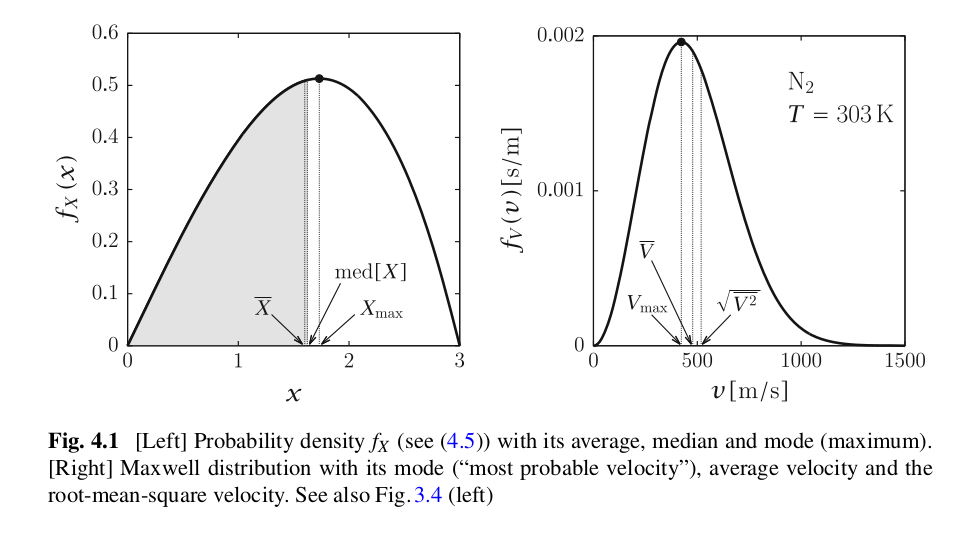
\includegraphics[scale=0.41]{../slides/figures/mean_median_mode_sirca.png}
\end{figure}
  
  
\subsection{Medidas de dispersión}

Independientemente de la medida de tendencia central que utilicemos en una
aplicación particular, también es importante conocer la dispersión de la
distribución. Estas medidas se encargan de mostrar que tan juntos o separados se
encuentran los datos de una distribución.

\begin{figure}[h!]
  \centering
  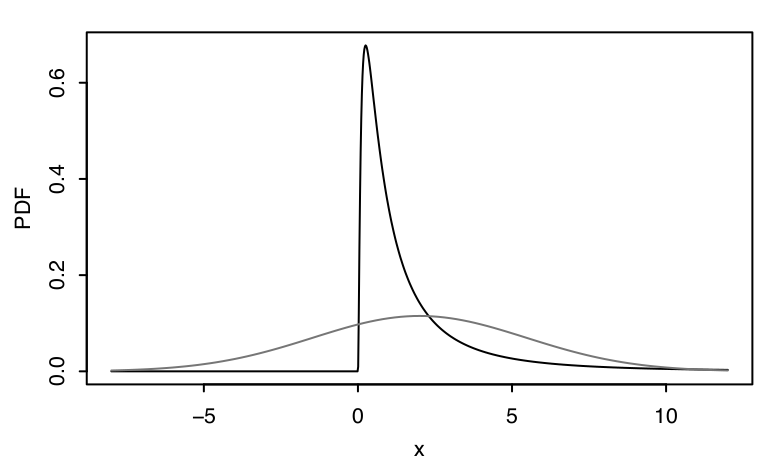
\includegraphics[scale=0.5]{../slides/figures/dispersion.png}
  \caption{Dos funciones de densidad de probabilida con media 2 y varianza 12. La
  curva de color claro es normal y simétrica, mientras que la más oscura es ua
  Log-Normal sesgada a la derecha.}
\end{figure}

\subsubsection{Tipos de momentos}

Sea $X$ una v.a. con media $\mu$ y varianza $\sigma$. Para cualquier entero
positivo $k$:

\begin{itemize}
  \item el $k$-ésimo momento de $X$ es $E(X^k)$.
  \item el $k$-ésimo momento central de $X$ es $E(X-\mu)^k$.
  \item el $k$-ésimo momento estandarizado de $X$ es $E(\frac{X-\mu}{\sigma})^k$.
\end{itemize}

La cantidad $X-\mu$ se llama desviación de una observación respecto a su media.
Como estas desviaciones se elevan al cuadrado y después se promedian, $\sigma^2$
será mucho menor para un conjunto de valores $x$ que estén cercanos a $\mu$, que
para un conjunto de valores que varíe de forma considerable de $\mu$.

El término momento viene de la física. 
  
\begin{figure}[h!]
  \centering
  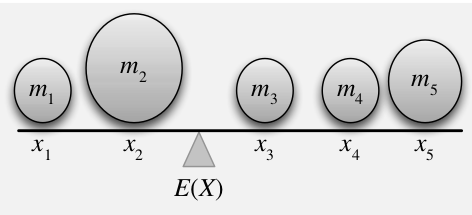
\includegraphics[scale=0.5]{../slides/figures/physics_moment.png}
    \caption{La media (primer momento) de una v.a. corresponde al centro de masa, y
    la varianza (segundo momento central) corresponde al momento de inercia con
    respecto al centro de masa.}
\end{figure}
  
\subsubsection{Momentos de una v.a.}

Los momentos de una variable aleatoria son cantidades que reflejan ciertas
características de un conjunto de datos numérico y se definen de la
siguiente manera:
  
\begin{itemize}
\item $E(X)$ también se le denomina como primer momento. También se puede
denotar como $\bar{X}$ o $\mu_{X}$, que implican una \textit{operación de
promedio} sobre la variable $X$.
\item $E(X^2)$. El segundo momento o varianza, denotado como $Var(X)$,
$\sigma_{X}^{2}$, o simplemente $\sigma^{2}$.
\item $E(X^3)$. El tercer momento es una medida de la asimetría
(\textit{skewness}).\\
\item $E(X^4)$. El cuarto momento o curtuosis es una medida de la altura de la
función de distribución de probabilidad.\\
  ...\\
  \item $E(X^k)$ es el $k$-ésimo momento.
\end{itemize}
  
Sean $x_1,...,x_n$ las observaciones de una variable cuantitativa y sea $k \geq
1$ un entero.

El $k$-ésimo momento está dado por el promedio aritmético de cada uno de los
datos, elevados a la potencia $k$.

\begin{equation}
  m_{k}^{'} = \frac{1}{n} \sum_{i=1}^{n} x_{i}^{k}
\end{equation}

Por ejemplo, para $k=1$, que es el primer momento o media del conjunto de datos, tenemos:

\begin{equation}
  m_{1}^{'} = \frac{1}{n} \sum_{i=1}^{n} x_{i}
\end{equation}
  
Por ejemplo, para $k=2$, que es el segundo momento, tenemos:

\begin{equation}
  m_{2}^{'} = \frac{1}{n} \sum_{i=1}^{n} x_{i}^{2}
\end{equation}
  
\subsubsection{Tipos de momentos}
Sea $X$ una v.a. con media $\mu$ y varianza $\sigma$. Para cualquier entero
positivo $k$:
  
\begin{itemize}
  \item el $k$-ésimo momento de $X$ es $E(X^k)$.
  \item el $k$-ésimo momento central de $X$ es $E(X-\mu)^k$.
  \item el $k$-ésimo momento estandarizado de $X$ es $E(\frac{X-\mu}{\sigma})^k$.
\end{itemize}
  
La cantidad $X-\mu$ se llama desviación de una observación respecto a su media.
Como estas desviaciones se elevan al cuadrado y después se promedian, $\sigma^2$
será mucho menor para un conjunto de valores $x$ que estén cercanos a $\mu$, que
para un conjunto de valores que varíe de forma considerable de $\mu$.
  
\subsection{Momento central}

Además, si $\bar{x}$ es la media, el $k$-ésimo momento central es:

\begin{equation}
  m_{k} = \frac{1}{n} \sum_{i=1}^{n} (x_{i} - \bar{x})^k
\end{equation}

Así, para $k=1$, tenemos:
\begin{equation}
  m_{1} = \frac{1}{n} \sum_{i=1}^{n} (x_{i} - \bar{x}) = 0
\end{equation}

  Para $k=2$, tenemos:
\begin{equation}
  m_{2} = \frac{1}{n} \sum_{i=1}^{n} (x_{i} - \bar{x})^2 = 0
\end{equation}

Así la varianza es el segundo momento central, y esta es una medida de la
dispersión de los datos.
  
No se conocen las características asociadas a cada uno de los momentos. Podemos
calcularlos y manipularlos matemáticamente pero no sabemos lo que representa el
séptimo momento de un conjunto de datos.

La curtosis y el coeficiente de asimetría se definen en términos de los momentos.


\subsubsection{Esperanza}

Sea $X$ una variable aleatoria discreta con función de probabilidad $f(x)$, que
puede tomar los valores $x_i=(i=1,2,...)$.\\

Entonces, se define el primer momento o esperanza de $X$, como la suma sobre todos los posibles
valores que la variable aleatoria puede tomar de $X$ por la probabilidad $P(X=x_i)=f_{X}(x_i)$.

\begin{equation}
  \bar{X} = E(X) = \sum_{i=1}^{n} x_i \cdot P(X=x_i)
  \label{eq:esperanza_discreta}
\end{equation}

Siempre y cuando esta suma sea finita.

\begin{equation}
  \sum_{x} |x| f(x) < \infty
\end{equation}

Si la variable aleatoria es continua, entonces el valor esperado o esperanza se
denota de la siguiente manera:

\begin{equation}
  \bar{X} = E(X) = \int_{-\infty}^{\infty} x \cdot f_{X}(x) \ dx
\end{equation}

Siempre y cuando la función de densidad sea finita.

\begin{equation}
  \int x^r \cdot f_{X}(x) \ dx < \infty
\end{equation}

\textbf{Ejemplo}

Consideremos que $X$ es una v.a. discreta con función de probabilidad $f(x)$:

\begin{center}
\begin{tabular}{c|cccc}
  $x$     & 0 & 1 & 2 & 3 \\
  \hline
  $f(x)$  & $\frac{1}{4}$ & $\frac{1}{2}$ & $\frac{1}{8}$ & $\frac{1}{8}$
\end{tabular}
\end{center}
  
De acuerdo con la Ec. (\ref{eq:esperanza_discreta}), tendremos:

\begin{equation}
  E(X) = 0 \cdot \frac{1}{4} + 1 \cdot \frac{1}{2} + 2 \cdot \frac{1}{8} + 3 \cdot \frac{1}{8} = \frac{9}{8}
\end{equation}
  
Sea una variable aleatoria $X$ cuya función de densidad es $f(x)=3x^2$ si $0
\leq x \leq 1$ y $0$ para el resto.

Para calcular $E(x)$:

\begin{equation}
  \begin{array}{rl}
    E(X)  & = \int_{- \infty}^{0} x \cdot 0 \ dx + \int_{0}^{1} x \cdot 3x^2 \ dx + \int_{1}^{\infty} x \cdot 0 \ dx \\
    \\
          & = \int_{- \infty}^{0} 0 \ dx + \int_{0}^{1} 3x^3 \ dx + \int_{1}^{\infty} 0 \ dx \\
    \\
          & = \int_{0}^{1} 3x^3 \ dx = 3 \ \int_{0}^{1} x^3 \ dx \\
    \\
          & = 3 \frac{x^4}{4} |_{0}^{1} = 3(\frac{1}{4} - \frac{1}{4}) = \frac{3}{4}
  \end{array}
\end{equation}
  
En resumen:
\begin{itemize}
\item El momento central de primer orden es cero $\mu = 0$

  
\item El segundo momento central o Varianza, está dado por:
Sea $X$ una v.a. con distribución de probabilidad $f(x)$ y media $\mu$. La
varianza de $X$ es:

\begin{equation}
  \sigma^2 = E[(X-\mu)^2] = \sum_{x}(x-\mu)^2 \ f(x)
\end{equation}
Si $X$ es discreta, y 

\begin{equation}
  \sigma^2 = E[(X-\mu)^2] = \int_{-\infty}^{\infty}(x-\mu)^2 \ f(x) \ d(x)
\end{equation}
Si $X$ es continua.

\item El tercer momento o asimetría (\textit{skewness}) de una v.a. $X$ con
media $\mu$ y varianza $\sigma^2$ es el tercer momento estandarizado de $X$:
  
\begin{equation}
  \text{Skew}(X) = E(\frac{X-\mu}{\sigma})^3
\end{equation}
  
Al estandarizar o normalizar primero, hacemos que la definición de Skew$(X)$ no
dependa de la ubicación o la escala de $X$, lo cual es razonable dado que ya
tenemos $\mu$ y esta nos proporciona información sobre la ubicación ($\mu = 0$ y
$\sigma^2 = 1$).

Decimos que una v.a. $X$ tiene una distribución simétrica con respecto a $\mu$
si $X-\mu$ tiene la misma distribución que $\mu-X$.

Una asimetría positiva es un indicativo de que la distribución tiene una cola
derecha más larga, comparada con la izquierda. 
  
    \begin{figure}[h!]
      \centering
      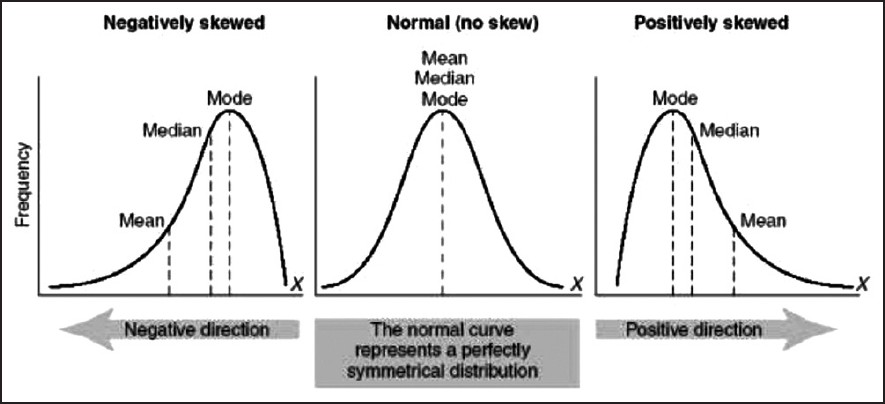
\includegraphics[scale=0.5]{../slides/figures/different_skewness.png}
    \end{figure}
  
\item El cuarto momento o curtuosis de una v.a. $X$ con media $\mu$ y varianza
$\sigma^2$ es el grado del decaimiento, suave o abrupto de la función de
distribución de probabilidad con respecto a la distribución normal (razon por la
cual se le resta 3).
  
  \begin{equation}
    \text{Kurt}(X) = E(\frac{X-\mu}{\sigma})^4 \ -3
  \end{equation}

    \begin{itemize}
      \item Para la distribución normal, $\text{Kurt}(X)=0$. A esta se le llama curva
            \textit{mesocúrtica}.
    \end{itemize}

    \begin{itemize}
    \item Cuando la curtuosis es positiva $\text{Kurt}(X)>0$ no indica que la
    distribución tiene un pico más prominente y que las colas decaen más
    abruptamente (curva \textit{leptocúrtica}).
    \item Cuando la curtuosis es negativa $\text{Kurt}(X)<0$ nos indica que el pico
    es menos pronunciado y que las colas son más fuertes (curva \textit{platicúrtica}).
      \end{itemize}

    \begin{figure}[h!]
      \centering
      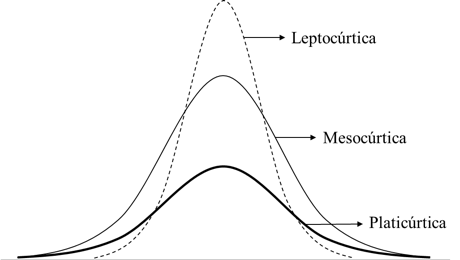
\includegraphics[scale=1]{../slides/figures/curtuosis.png}
    \end{figure}

\end{itemize}

